\section[Differenzierbare Abbildungen, Taylorentwicklung]{Differenzierbare Abbildungen, Verkettung, Taylorentwicklung, lokale Extrema}
\Einleitung{Wir erweitern unser Versändnis von Abbildungen, die aus $U\subseteq\mathbb{R}^n$ in den $\mathbb{R}^m$ abbilden.\\
Als Bedingung für deren Differenzierbarkeit hatten wir letzte Woche festgelegt, dass mit $\xivec\in U\setminus\MengeDirekt{\Vec{0}}$ der Grenzwert $\lim_{\Norm{\xivec}\to0}\frac{\Norm{\Fvec(\xvec-\xivec)-\Fvec(\xvec)-A(\xivec)}}{\Norm{\xivec}}=0$ sein muss, damit $\Fvec:U\to\mathbb{R}^m$ in $\xvec\in U$ total differenzierbar ist.\\
Dafür muss die lineare Abbildung $A:U\to\mathbb{R}^m$ existieren, welche wir als Analogon der Ableitung für die Differenzierbarkeit in 1D entdeckt hatten.\\
Deren darstellende Matrix ist die Jacobi-Matrix, die durch $J_\xvec=\MatrixInline{\grad(F_1(\xvec))^T\\\grad(F_2(\xvec))^T\\\grad(F_3(\xvec))^T}$ berechnet werden kann.\\
Zudem wurde gezeigt, dass $\Fvec$ differenzierbar ist, falls alle partiellen Ableitungen der Komponentenfunktionen existieren und stetig sind.\\
Diese Woche erarbeiten wir uns die zugehörigen Werkzeuge, die wir größtenteils schon von Funktionen $f:\mathbb{R}\to\mathbb{R}$ kennen, und erweitern sie auf $\Fvec:U\to\mathbb{R}^m$. Einige davon ergeben nur Sinn falls $m=1$, also aufpassen!}

\subsection{Rechenregeln für das Differential}
\begin{Satz}
{Rechenregeln}{Regeln für das Differential}
Für eine Abbildung $\Fvec:\mathbb{R}^n\to\mathbb{R}^m$, die in $\xvec\in\mathbb{R}^n$ differenzierbar ist, gelten folgende Regeln für das Differential $d\Fvec_\xvec$:
\begin{enumerate}
    \item \textbf{Linearität}:\\
    Für $\Gvec:\mathbb{R}^n\to\mathbb{R}^m$, das in $\xvec$ differenzierbar ist, und $\lambda\in\mathbb{R}$ gilt
    \begin{equation*}
        \boxed{d(\lambda\Fvec+\Gvec)_\xvec=\lambda d\Fvec_\xvec+d\Gvec_\xvec}.
    \end{equation*}
    \item \textbf{Produktregel mit skalarer Funktion}:
    Für $h:\mathbb{R}^n\to\mathbb{R}$, das in $\xvec$ differenzierbar ist, gilt:
    \begin{equation*}
        \boxed{d(h\Fvec)_\xvec=\Fvec(\xvec)dh_\xvec+h(\xvec)d\Fvec_\xvec}.
    \end{equation*}
    \item \textbf{Quotientenregel mit skalarer Funktion}:\\
    Für $g:\mathbb{R}^n\to\mathbb{R}$, das in $\xvec$ differenzierbar ist mit $g(\xvec)\neq0$, gilt:
    \begin{equation*}
        \boxed{d\BracedIn{\frac{1}{g}\Fvec}_\xvec=\frac{1}{g^2(\xvec)}(g(\xvec)d\Fvec_\xvec-\Fvec(\xvec)dg_\xvec}.
    \end{equation*}
\end{enumerate}
\end{Satz}
\blue{Wie auch bei 1D-Funktionen liefert uns die Kettenregel eine Rechenvorschrift für das Differential verketteter Abbildungen.\\
Hierbei müsst ihr immer genau auf die Dimensionen der Räume achten!}
\begin{Satz}
{Rechenregel}{Kettenregel}
Für $\textcolor{orange}{U\subseteq \mathbb{R}^n}$, $\textcolor{mygreen}{V\subseteq\mathbb{R}^m}$ offen, $\Fvec:\textcolor{orange}{U}\to\textcolor{mygreen}{\mathbb{R}^m}$ mit $\textcolor{mygreen}{\Fvec(U)\subseteq V}$ und $\Gvec:\textcolor{mygreen}{V}\to\textcolor{red}{\mathbb{R}^k}$ gilt, falls $\Fvec$ differenzierbar in $\textcolor{orange}{\xvec\in U}$ und $\Gvec$ differenzierbar in $\textcolor{mygreen}{\yvec=\Fvec(\xvec)\in V}$ ist, dass deren Verkettung $\Gvec\circ\Fvec: \textcolor{orange}{U}\to\textcolor{red}{\mathbb{R}^k}$ in $\textcolor{orange}{\xvec}$ differenzierbar ist und für das Differential
\begin{equation}
    d(\Gvec\circ\Fvec)_{\textcolor{orange}{\xvec}}= d\Gvec_{\textcolor{mygreen}{\Fvec(\xvec)}}\circ d\Fvec_{\textcolor{orange}{\xvec}}
\end{equation}
\end{Satz}
\blue{Das schreit doch nach einem Beispiel, oder?}
\begin{Beispiel}{Zur Kettenregel}
Seien $\Fvec:\mathbb{R}^2\to\mathbb{R}^3,\,(x,y)\mapsto\MatrixInline{y\sin(x)\\2\sqrt[3]{y^2}x\\y^2\cos^2(x)}$ und $G:\mathbb{R}^3\to\mathbb{R},\,(x,y,z)\mapsto x^2+y^3+z$.\\
Eine Verkettung ergibt die Funktion
\begin{align*}
    G\circ\Fvec:\mathbb{R}^2\to\mathbb{R},\,(G\circ\Fvec)(x,y)&=G(\Fvec(x,y))=G\Matrix{y\sin(x)\\2\sqrt[3]{y^2}x\\y^2\cos^2(x)}\\
    &=y^2\sin^2(x)+8y^2x^3+y^2\cos^2(x)=y^2(1+8x^3).
\end{align*}
Wir betrachten die Jacobi-Matrizen:
\begin{align*}
    d\Fvec_\xvec&=J_\xvec(\Fvec)=\Matrix{\grad(F_1)^T\\\grad(F_2)^T\\\grad(F_3)^T}=\Matrix{y\cos(x)&\sin(x)\\2\sqrt[3]{y^2}&4/3 xy^{-\frac{1}{3}}\\-2y^2\sin(x)\cos(x)&2y\cos^2(x)}\\
    d G_\xvec&=J_\xvec(G)=\Matrix{\grad(G_1)^T}=\Matrix{2x&3y^2&1}\\
    d(G\circ \Fvec)_\xvec&=\Matrix{\grad((G\circ\Fvec)_1)^T}=\Matrix{24x^2y^2&2y(1+8x^3)}.
\end{align*}
Das war also die direkte Berechnung. Nun wenden wir die Kettenregel an:
\begin{eqnarray*}
    d G_{\Fvec(\xvec)}\circ d\Fvec_\xvec&\overset{\footnote{Die Verkettung linearer Abbildungen kann über Multiplikation der darstellenden Matrizen durchgeführt werden.}}{=}&\Matrix{2y\sin(x)&3(2\sqrt[3]{y^2}x)^2&1}\Matrix{y\cos(x)&\sin(x)\\2\sqrt[3]{y^2}&4/3xy^{-\frac{1}{3}}\\-2y^2\sin(x)\cos(x)&2y\cos^2(x)}\\
    &=&\Matrix{(2y^2-2y^2)\sin(x)\cos(x)+24y^{\frac{6}{3}}x^2&2y\sin^2(x)+16y^{\frac{4}{3}-\frac{1}{3}}x^3+2y\cos^2(x)}\\
    &=&\Matrix{24y^2x^2&2y(1+8x^3)}.
\end{eqnarray*}
Die Kettenregel funktioniert also wie erwartet.
\end{Beispiel}
\begin{Satz}
{Satz}{Kettenregel in Komponenten}
Mit denselben Voraussetzungen wie eben und $H:G\circ\Fvec:\textcolor{orange}{U}\to\textcolor{red}{\mathbb{R}^k}$ gilt für die Komponenten $\textcolor{orange}{i=1,\ldots,n}$ und $\textcolor{red}{l=1,\ldots,k}$:
\begin{equation}
    \partial_iH_l(\textcolor{orange}{\xvec})=\sum_{j=1}^{\textcolor{mygreen}{m}}\partial_jG_l(\textcolor{mygreen}{\Fvec(\textcolor{orange}{\xvec})})\partial_iF_j(\textcolor{orange}{\xvec}).
\end{equation}
\end{Satz}
\blue{Dies entspricht nur einer komplizerteren Schreibweise.\\
In unserem Beispiel war z. B. $\partial_xH_1(\xvec)=24x^2y^2$ und $\partial_yH_2(\xvec)=2y(1+8x^3)$.\\
Ich (Fabian) präferiere die obere Art für direkte Rechnungen.}
\begin{Beispiel}
{Verkettung von Spur und Quadrat für Matrizen}
Wir können für die Abbildungen $F:\Met(n,\mathbb{R})\to\Met(n,\mathbb{R}),\,A\mapsto A^2$ und $G:\Met(n,\mathbb{R})\to\mathbb{R},\, A\mapsto\Tr(A)$ ebenfalls das Differential der Verkettung $G\circ F$ einer Matrix $B\in\Met(n,\mathbb{R})$ im Punkt $A\in\Met(n,\mathbb{R})$ bestimmen, denn $F$ und $G$ sind in $A$ differenzierbar mit
\begin{eqnarray*}
    d F_A(B)&=&\diff{}{t}\big|_{t=0}\BracedInSqr{\BracedIn{A+tB}^2}\overset{\footnote{Wie bei der Richtungsableitung fassen wir die Ableitung als infinitesimale Verschiebung in $B$-Richtung auf.\\
    Wir wenden zudem die Produktregel an.}}{=}\BracedInSqr{\diff{}{t}(A+tB)(A+tB)+(A+tB)\diff{}{t}(A+tB)}_{t=0}\\
    &=&\BracedInSqr{B(A+tB)+(A+tB)B}_{t=0}=BA+AB\\
    dG_A(B)&=&\diff{}{t}\big|_{t=0}\BracedInSqr{\Tr(A+tB)}=\diff{}{t}\BracedInSqr{\sum_{i=1}^n\BracedIn{a_{ii}+tb_{ii}}}_{t=0}\\
    &\overset{\footnote{Linearität}}{=}&\sum_{i=1}^nb_ii=\Tr(B)
\end{eqnarray*}
Daraus folgt, dass $G\circ F:\Met(n,\mathbb{R})\to\mathbb{R},\,A\mapsto \Tr(A^2)$ differenzierbar mit
\begin{equation*}
    d(G\circ F)_A(B)=d G_{F(A)}\circ dF_A(B)=\Tr(AB+BA)\overset{\footnote{Die Spur ist linear und es gilt $\Tr(AB)=\Tr(BA)$}}{=}2\Tr(AB).
\end{equation*}
\end{Beispiel}

\subsection[Verschiedene alte Bekannte erweitert auf den R hoch n]{Verschiedene alte Bekannte erweitert auf den $\mathbb{R}^n$}
\begin{Wiederholung}
{Mittelwertsatz}
\begin{wrapfigure}{r}[0pt]{.23\textwidth}
 \vspace{-15pt}
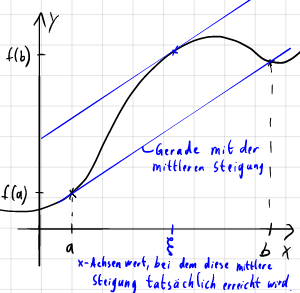
\includegraphics[width=.23\textwidth]{Dateien/08/09Mittelwertsatz.PNG}
 \vspace{-15pt}
\end{wrapfigure}
Ist $f:[a,b]\to\mathbb{R}$ stetig und differenzierbar auf $(a,b)$, so existiert ein\\
$\xi\in(a,b)$, sodass $f'(\xi)=\frac{f(b)-f(a)}{b-a}$.\\
\blue{Anschaulich:\\
Für stetige und differenzierbare Funktionen gibt es für jedes Intervall $(a,b)$ mindestens einen Punkt, in dem die \underline{lokale Steigung} gleich der \underline{mittleren Steigung} ist.}
\end{Wiederholung}
\begin{Satz}
{Satz}{Mittelwertsatz für Funktionen im $\mathbb{R}^n$}
Für stetig differenzierbare Funktionen $F:U\to\mathbb{R}$ ($U\subseteq\mathbb{R}^n$ offen), $\xvec\in U$ und $\xivec\in U$ mit $(\xvec+t\xivec)\in U\,\forall t\in[0,1]$ existiert $\xvec_0\in \xvec+t_0\xivec\in U$ mit $t_0\in(0,1)$, sodass
\begin{equation}
    F(\xvec+\xivec)-F(\xvec)=dR_{\xvec_0}(\xivec).
\end{equation}
\end{Satz}
\blue{Erläuterung zum Mittelwertsatz:
\begin{center}
    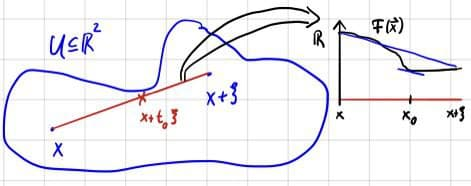
\includegraphics[width=.5\textwidth]{Dateien/08/08Mittelwertsatz.jpg}
\end{center}
Unsere \textit{Intervallgrenzen} $a$ und $b$ des bekannten Mittelwertsatzes wurden nun ersetzt durch die gerade Verbindungslinie zwischen $\xvec$ und $\xivec$.\\
Die Aussage bezieht sich nun im Prinzip auf das Differential ($\overset{\wedge}{=}$ Steigung) entlang dieser Geraden.\\
Salopp geschrieben: Seien $\xvec_1$ und $\xvec_2$\footnote{wobei $\xvec_2=\xvec_1+\xivec$}$\in U$ und $F$ definiert wie oben, so existiert $\xvec_0\in\Vec{x_1x_2}$\footnote{Hiermit ist die Verbindungslinie zwischen $\xvec_1$ und $\xvec_2$ gemeint}, sodass $F(\xvec_2)-F(\xvec_1)=\BiFo{\grad(F(\xvec_0)),(\xvec_2-\xvec_1)}$ ist.\footnote{Für Abbildungen nach $\mathbb{R}$ ist die Jacobi-Matrix ja schlicht der Gradient, die Multiplikation kann mithilfe des Skalarproduktes ausgedrückt werden.}\\
Dies können wir nun wieder so deuten, dass die Sekantensteigung zwischen $F(\xvec_1)$ und $F(\xvec_2)$ mindestens einmal auf der Verbindungsstrecke auftritt.\\
Der Mittelwertsatz ist z. B. geeignet, um Lipschitz-Stetigkeit (definiert ihr noch) zu zeigen.\\
Zudem ist er zentral für die gleich folgende Aussage über die Lösung der DG $dF_\xvec=0\,\forall \xvec\in U$.}
\begin{Def}
{Wegzusammenhang}
Wir nennen $U\subseteq\mathbb{R}^n$ \red{wegzusammenhängend}, falls es für je zwei Punkte $\xvec,\yvec\in U$ stets eine \underline{stetige Kurve} $x:[0,1]\to U$ mit $c(0)=\xvec$ und $c(1)=\yvec$ gibt.\\
\blue{Diese kann man sich sehr leicht anschaulich merken:}
\begin{center}
    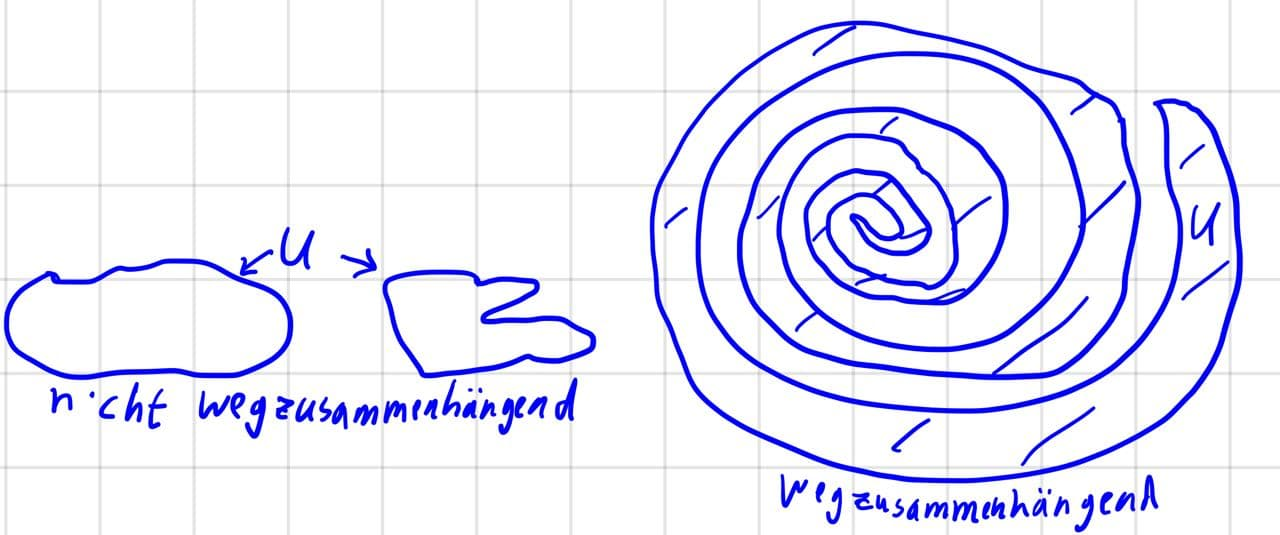
\includegraphics[width=.45\textwidth]{Dateien/08/08Wegzusammenhang.jpg}
\end{center}
\end{Def}
\begin{Satz}
{Satz}{Verschwindendes Differential impliziert konstante Abbildung}
Ist $U\subseteq\mathbb{R}^n$ wegzusammenhängend und $\Fvec:U\to\mathbb{R}^m$ differenzierbar mit $d\Fvec_\xvec=0\,\forall\xvec\in U$, so ist $\Fvec$ eine konstante Abbildung.\footnote{Diesen Satz hatten wir auch schon in 1D kennengelernt: Für stetige, differenzierbare Funktionen mit $f(x)=0\,\forall x\in (a,b)$ folgt, dass diese konstant sind.}
\end{Satz}
\begin{Def}
{Niveaumengen}
Für eine offene TM $U\subseteq\mathbb{R}^n$ und eine stetig differenzierbare Abbildung $F:U\to\mathbb{R}$ nennen wir
\begin{equation}
    N_f(k):=\Menge{\xvec\in U}{f(\xvec)=k}\quad\tx{mit } k\in\mathbb{R}
\end{equation}
eine \red{Niveaumenge}.\\
\blue{Diese ist also ein Zusammenschluss von Punkten aus dem Urbildraum, für die $f(x)$ den gleichen Wert $k\in\mathbb{R}$ annimmt.\\
In der Physik nennen wir so etwas für Kraftfelder auch \red{Äquipotentiallinie}.}
\end{Def}
\begin{Satz}
{Satz}{Zu Niveaumengen}
$\grad f$ steht senkrecht auf Niveaumengen, d. h. für alle differenzierbaren Kurven $c:(a,b)\to\mathbb{R}^n$, die innerhalb der Niveaumenge $N_f(k)$ verlaufen, gilt:
\begin{equation}
    \grad f\big|_{c(t)}\perp c'(t)\quad \forall t\in (a,b).
\end{equation}
\blue{In der folgenden Skizze haben wir eine Anschauung versucht:}
\begin{center}
    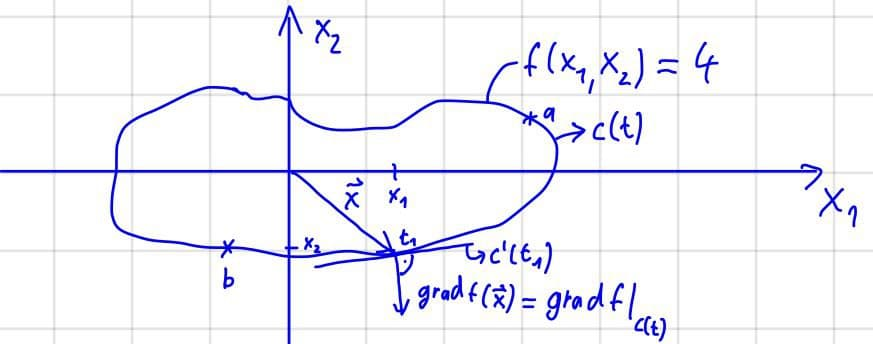
\includegraphics[width=.5\textwidth]{Dateien/08/08Aequipotential.jpg}
\end{center}
\blue{Vergleichen wir dies wieder mit der Physik, so identifizieren wir hiermit die Aussage, dass entlang von Äquipotentiallinien keine Arbeit verrichtet wird. Stellt euch vor, ihr seid auf einem Berg. Geht ihr nach unten oder nach oben, müsst ihr Arbeit im Gravitationsfeld verrichten, weil ihr gegen $\Fvec=-\grad V$ arbeitet. Bleibt ihr hingegen auf einer Höhe, bleibt euer 'Potential' konstant.}
\end{Satz}
\subsubsection{Extrema auf \textit{U}}
Auch lokale Extrema werden wieder analog zu den 1D-Funktionen\\
(Maximum in $z\iff\exists \epsilon>0: f(z)\geq f(\zeta)\,\forall\zeta\in D$ mit $\Abs{\zeta-z}<\epsilon$) für Funktionen auf dem $\mathbb{R}^n$ definiert:
\begin{Def}
{Lokale Extrema}
\begin{wrapfigure}{r}[0pt]{.25\textwidth}
 \vspace{-15pt}
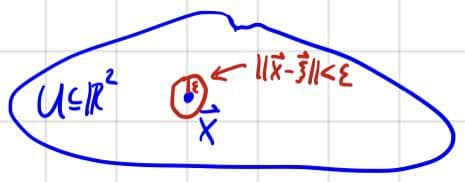
\includegraphics[width=.25\textwidth]{Dateien/08/08Extremum.jpg}
 \vspace{-15pt}
\end{wrapfigure}
Sei $U\subseteq\mathbb{R}^n$ offen, $f:U\to\mathbb{R}$ und $\xvec\in U$.\\
Falls es $\epsilon>0$ gibt, sodass
\begin{equation}
    f(\xvec)\geq f(\xivec)\quad\forall\xivec\in U \tx{ mit }\Norm{\xvec-\xivec}<\epsilon,
\end{equation}
sagen wir, dass $f$ ein \red{lokales Maximum} in $\xvec$ hat (bzw. Minimum für $f(\xvec)\leq f(\xivec)$.\\
Bei \underline{echter} Ungleichheit (d. h. $f(\xvec)\neq f(\xivec)\,\forall\xivec\in U\setminus\MengeDirekt{\Vec{x}}$ mit $\Norm{\xvec-\xivec}<\epsilon$) nennen wir das Extremum \red{isoliert}.
\end{Def}
\blue{Wir definieren Extrema also, indem wir sagen, dass die von der $\epsilon$-Umgebung $V:=\Norm{\xvec-\xivec}<\epsilon$ des Urbildraumes erzeugte Umgebung $f(V)$ des Bildraumes keine 'höheren' bzw. 'niedrigeren' Werte hat.}\\
Im $\mathbb{R}^m$ haben wir keine Ordnungsrelationen definiert, weshalb das Konzept des Extremums für Funktionen $\Fvec:\mathbb{R}^n\to\mathbb{R}^m$ für $m>1$ keinen Sinn ergibt (zumindest in dieser Form).

\begin{Satz}
{Satz}{Notwendiges Kriterium für Extrema}
Falls $F:U\to\mathbb{R}$ partiell differenzierbar in $\xvec\in U$ ist \underline{und} dort ein lokales Extremum annimmt, so folgt:
\begin{equation}
    \boxed{\grad (f(\xvec))=0}.
\end{equation}
\end{Satz}
\red{Achtung: Wie auch bei $f'(x)=0$ ist auch dies nicht hinreichend für Extrema. Wir benötigen noch eine Art zweite Ableitung dafür:}
\begin{Def}
{Hessematrix}
Für zweifach stetig differenzierbare Funktionen $f:\mathbb{R}^n\to\mathbb{R}$ nennen wir die symmetrische Matrix der zweiten Ableitungen die \red{Hesse-Matrix}
\begin{equation}
    \Hess( f(\xvec))=\Matrix{\partial_1\partial_1 f(\xvec)&\cdots&\partial_1\partial_n f(\xvec)\\
    \vdots&\ddots&\vdots\\\partial_n\partial_1 f(\xvec)&\cdots&\partial_n\partial_nf(\xvec)}.
\end{equation}
\end{Def}
\blue{Dies entspricht der zweiten Ableitung, die wir von 1D-Funktionen kennen. Allerdings können wir hier nicht einfach die Krümmung am Vorzeichen \underline{einer} zweiten Ableitung festmachen, wir müssen das ein bisschen verallgemeinern.\\
Dafür benötigen wir den Begriff der Definitheit:}
\begin{Def}
{Definitheit}
Für \underline{symmetrische Bilinearformen} $\beta$ (die ja mit darstellender Matrix $A$ über\\
$\beta(v,w)=\BiFo{v,Aw}$ auf euklidischen Vektorräumen mithilfe des Skalarprodukts dargestellt werden können) führen wir neben dem Begriff
\begin{itemize}
    \item der \red{positiven Definitheit} ($\beta(v,v)>0\,\forall v\in V\setminus\MengeDirekt{0}$,
    \item die \red{negative Definitheit} ($\iff-\beta$ ist positiv definit)
    \item und die \red{pos./neg. semi-Definitheit} ($\beta(v,v)\gtreqless 0\,\forall v\in V$) ein.
\end{itemize}
Ist $\beta$ weder positiv noch negativ definit, nennen wir $\beta$ \red{indefinit}.
\end{Def}
\blue{Damit können wir nun symmetrische Endomorphismen (und somit auch die Hesse-Matrix) klassifizieren.\\
Ihr habt allerdings keine Sätze kennengelernt, um Definitheit wirklich zu zeigen. Dazu hier nur so viel:}
\begin{Satz}
{Satz}{Definitheit mithilfe der Eigenwerte (nicht im Skript)}\label{satz:08DefinitheitEigenwerte}
Eine symmetrische Matrix $A$ ist
\begin{itemize}
    \item positiv definit, wenn alle Eigenwerte $\lambda_i>0$ sind,
    \item negativ definit, wenn alle Eigenwerte $\lambda_i<0$ sind und
    \item indefinit, wenn es sowohl positive als auch negative Eigenwerte gibt.
\end{itemize}
Dieses Kriterium folgt quasi aus der Diagonalisierbarkeit und der Tatsache, dass sich die Definitheit unter Basistransformation nicht ändert.
\end{Satz}
Es gibt noch andere, angenehmere Kriterien wie z. B. das \red{Hauptminorenkriterium}, aber das kennt ihr nicht aus der Vorlesung.
\begin{Satz}
{Satz}{Hinreichendes Kriterium für Extrema}
Ist $f:U\to\mathbb{R}$ zweimal stetig differenzierbar, so gilt:
\begin{itemize}
    \item $\grad(f(\avec))=0\land \Hess(f(\avec))$ positiv \underline{semi}-definit $\impliedby$ $f$ hat ein \underline{lokales} Minimum in $\avec\in U$.
    \item $\grad(f(\avec))=0\land \Hess(f(\avec))$ positiv definit $\iff$ $f$ hat ein \underline{isoliertes} Minimum in $\avec\in U$.\footnote{Vergleiche $f'(a)=0\land f''(a)>0\implies $ \Smiley[1]}
    \item Analog für negative (semi-)Definitheit und lokale/isolierte Maxima.
\end{itemize}
Ist $\Hess (f(\avec))$ indefinit, hat $f$ in $\avec$ kein lokales Extremum.
\end{Satz}
\begin{Beispiel}
{Extrema einer 2D-Funktion}
\begin{wrapfigure}{r}[0pt]{.4\textwidth}
 \vspace{-15pt}
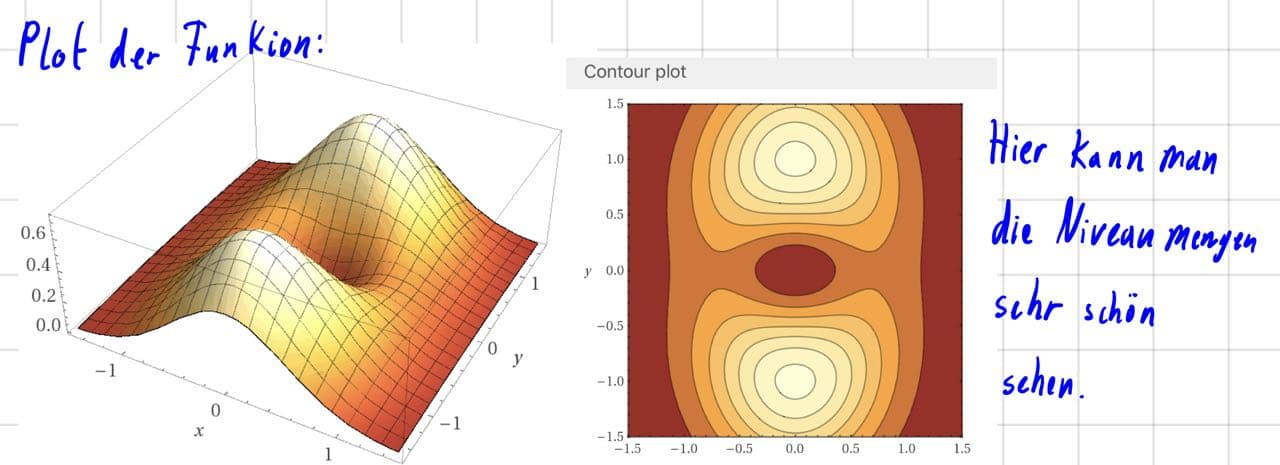
\includegraphics[width=.4\textwidth]{Dateien/08/08MinMaxFunk.jpg}
 \vspace{0pt}
\end{wrapfigure}
Wir untersuchen die Funktion
\begin{equation*}
    f:\mathbb{R}^2\to\mathbb{R},\,f(x,y)=(x^2+2y^2)e^{-2x^2-y^2}.
\end{equation*}
Diese ist zweimal stetig differenzierbar.\\
Wir bestimmen den Gradienten:
\begin{equation*}
    \grad(f(x,y))=\Matrix{\partial_xf(x,y)\\\partial_yf(x,y)}=-2e^{-2x^2-y^2}\Matrix{x(2x^2+4y^2-1)\\y(x^2+2y^2-2)}.
\end{equation*}
Wir setzen $\grad(f(x,y))=\Vec{0}$ und lösen nach $x$ und $y$ auf. Mit dem Satz über Nullteilerfreiheit ergeben sich die Gleichungen
\begin{align*}
    x(2x^2+4y^2-1)&=0\\
    y(x^2+2y^2-2)&=0.
\end{align*}
Wir machen eine Fallunterscheidung:
\begin{itemize}
    \item Für $x=0$:\\
    Entweder $y=0$ oder $2y^2-2=0\iff y=\pm 1$.
    \item Für $y=0$:\\
    Entweder $x=0$ oder $2x^2-1=0\iff x=\pm\frac{1}{\sqrt{2}}$.
    \item Für $x\neq0$ und $y\neq 0$:\\
    $2x^2+4y^2-1=0\iff x^2=\frac{1}{2}-2y^2$ setzen wir in die zweite Gleichung ein und erhalten
    $y\BracedIn{\frac{1}{2}-2y^2+2y^2-2}=0\iff-\frac{3}{2}y=0$ \Lightning (Widerspruch zu $y\neq0$)
\end{itemize}
Somit haben wir alle Nullstellen gefunden.\\
Für die Hesse-Matrix bestimmen wir alle gemischten zweiten partiellen Ableitungen:
\begin{align*}
    \partial_x\partial_xf(x,y)&=e^{-2x^2-y^2}\BracedIn{16x^4+4x^2(8y^2-5)-8y^2+2}\\
    \partial_y\partial_yf(x,y)&=e^{-2x^2-y^2}\BracedIn{x^2(4y^2-2)+8y^4-20y^2+4}\\
    \partial_x\partial_yf(x,y)&=e^{-2x^2-y^2}4xy\BracedIn{2x^2+4y^2-5}\\
    \partial_y\partial_xf(x,y)&=\partial_x\partial_yf(x,y).
\end{align*}
Wir sparen uns, dies als Matrix $\Hess(f(x,y))$ aufzuschreiben und führen die Tests (mithilfe von \hyperref[satz:08DefinitheitEigenwerte]{Satz 8.8}) für die gefundenen Nullstellen $\vvec_1=\MatrixInline{0\\0},\,\vvec_{2,3}=\MatrixInline{0\\\pm1},\vvec_{4,5}=\MatrixInline{\pm1/\sqrt{2}\\0}$ durch:
\begin{align*}
    \Hess(f(0,0))&=\Matrix{2&0\\0&4}\implies \tx{positiv definit}\implies \tx{isoliertes Minimum.}\\
    \Hess(f(0,\pm1))&=e^{-1}\Matrix{-6&0\\0&-8}\implies \tx{negativ definit}\implies \tx{isolierte Maxima.}\\
    \Hess\BracedIn{\BracedIn{\pm\frac{1}{\sqrt{2}},0}}&=e^{-1}\Matrix{-4&0\\0&3}\implies \tx{indefinit}\implies \tx{keine Extrema.}
\end{align*}
\end{Beispiel}
\subsubsection{Taylorreihen auf \textit{U}}
Wir erinnern uns zurück an die 1D-Taylorentwicklung, bei der wir eine $k$-fach differenzierbare Funktion durch ein Polynom $k-1$-ten Grades approximiert haben und als Koeffizienten der $(x-x_0)^r$ die $r$-ten Ableitungen im Entwicklunspunkt $x_0$ geteilt durch $r!$ genutzt haben, sodass das Ganze so aussah:
\begin{Wiederholung}
{Taylorpolynom}
Für eine $k$-fach differenzierbare Funktionen $f:[a,b]\to\mathbb{R}$ nennen wir
\begin{equation*}
    T_k(f,x_0)(x)=\sum_{r=0}^k\frac{f^{(r)}(x_0)}{r!}(x-x_0)^r=f(x_0)+f'(x_0)(x-x_0)+\frac{1}{2!}f''(x_0)(x-x_0)^2+...
\end{equation*}
das \red{Taylorpolynom} der Ordnung $k$ von $f$ um den \red{Entwicklungspunkt} $x_0\in[a,b]$.
\end{Wiederholung}
Die Konvergenz der Reihe im Intervall $(a,b)$ gegen $f$ bei $k\to\infty$ konnten wir bestimmen, indem wir die Konvergenz des Restglieds überprüft haben:
\begin{Wiederholung}
{Restglied}
Der Fehler auf die Approximation für das Taylorpolynom $T_{k-1}$ von $(k-1)$-ter Ordnung kann z.B. durch das \red{Lagrangesche Restglied}
\begin{equation*}
    R_k(x)=\frac{f^{(k)}(\xi)}{k!}(x-x_0)^k
\end{equation*}
abgeschätzt werden, wobei $\xi\in(x_0,x)$ oder $\xi\in(x,x_0)$ und $\xi$ für alle $x\in[a,b]$ existiert, sodass $f(x)=T_{k-1}(x)+R_k(x)$ ist.
\end{Wiederholung}
\begin{Def}
{Polynome im $\mathbb{R}^n$}
Ein allgemeines Polynom \underline{$m$-ten Grades} $P:\mathbb{R}^n\to\mathbb{R}$ sieht für $n=2$\footnote{sonst wird's zu unübersichtlich - das lässt sich aber einfach auf höhere Dimensionen übertragen.} so aus:
\begin{equation}
    P(x,y)=\sum_{k+l\leq m}a_{kl}x^ky^l.
\end{equation}
\blue{Ein Polynom 2-ten Grades ($m=2$) ist somit durch
\begin{equation*}
    P(x,y)=a_{00}+a_{10}x+a_{01}y+a_{11}xy+a_{20}x^2+a_{02}y^2
\end{equation*}
gegeben.}
\end{Def}
\begin{Beispiel}
{Hinführung zum Taylorpolynom}
Das Taylorpolynom einer Funktion $F:\mathbb{R}^2\to\mathbb{R}$ um den Punkt $\xvec_0=\MatrixInline{x_0\\y_0}\in\mathbb{R}^2$ ist dann ganz analog zu 1D
\begin{equation*}
    T_m(F,\xvec_0)(x,y)=\sum_{k+l\leq m}a_{kl}(x-x_0)^k(y-y_0)^l.
\end{equation*}
Wie sehen aber die Koeffizienten $a_{kl}$ aus?\\
Wie in 1D wollen wir, dass diese genau den Ableitungen an der Entwicklungsstelle entsprechen.\\
Dafür betrachten wir die $i$-te Ableitung von $F$ in $x$-Richtung und die $j$-te in $y$-Richtung:
\begin{eqnarray*}
    \partial_x^{(i)}\partial_y^{(j)}F(x,y)\big|_{x_0,y_0}&=&\partial_x^{(i)}\partial_y^{(j)}\BracedIn{\sum_{k+l\leq m}a_{kl}(x-x_0)^k(y-y_0)^l}\big|_{x_0,y_0}\\
    &=&a_{ij}\cdot\underbrace{i(i-1)\cdots 1}_{\tx{Aus }\partial_x^{(i)}(x-x_0)^i}\cdot \underbrace{j(j-1)\cdots 1}_{\tx{Aus }\partial_y^{(j)}(y-y_0)^j}\underbrace{(x_0-x_0)^0(y_0-y_0)^0}_{\footnote{Hier setzen wir die Auswertung bei $x_0$ und $y_0$ schon ein und berücksichtigen, dass in diesem Kontext $0^0=1$ definiert ist.}} +\underbrace{0}_{\footnote{Die anderen Summanden haben entweder durch $(x_0-x_0)^n=0$ oder durch zu hohe Ableitungen den Faktor 0 im Produkt und verschwinden daher.}}
\end{eqnarray*}
Also sind die Koeffizienten des Polynoms sinnvoll durch 
\begin{equation*}
    a_{ij}=\frac{\partial_x^{(i)}\partial_y^{(j)}F(x_0,y_0)}{i!j!}
\end{equation*}
gegeben.\\
Wir können also $F:\mathbb{R}^2\to\mathbb{R}$ darstellen durch
\begin{equation}
    T_m(F,\xvec_0)(x,y)=\sum_{k+l\leq m}\frac{\partial_x^{(k)}\partial_y^{(l)}F(x_0,y_0)   }{k!l!}(x-x_0)^k(y-y_0)^l+\varphi(\xvec-\xvec_0),
\end{equation}
wobei wir das Restglied $\varphi$ noch sinnvoll definieren müssen.\\
\red{Anmerkung:}\\
Im Skript wird $\xivec\in\mathbb{R}^n$ genutzt, was aber mehr oder weniger einfach $\xivec=\xvec-\xvec_0$ ist.
\end{Beispiel}
\blue{Wir schauen uns den Spezialfall $m=2$ an:}
\begin{Satz}
{Satz}{Quadratisches Taylorpolynom}
Ist $U\subseteq\mathbb{R}^n$ offen, $f:U\to\mathbb{R}$ zweifach stetig differenzierbar und $\xvec_0,\xivec\in\mathbb{R}^n$, sodass die Verbindungsstrecke $\Menge{\xvec_0+t\xivec}{t\in[0,1]}\subseteq U$ zwischen $\xvec_0$ und $\xivec$ in $U$ enthalten ist.\\
Dann ist
\begin{equation}
    f(\xvec_0-\xivec)=\underbrace{f(\xvec_0)+ \sum_{i=1}^n\partial_if(\xvec_0)\xi_i+\frac{1}{2}\sum_{i,j=1}^n\partial_i\partial_jf(\xvec_0)\xi_i\xi_j}_{\tx{Quadratisches Taylorpolynom}}+\varphi(\xivec),
\end{equation}
wobei $\xvec_0$ also der Entwicklungspunkt und $\xivec$ die neue Variable sind.\\
Das Restglied $\varphi(\xivec)$ muss die Eigenschaft 
\begin{equation*}
    \lim_{\xivec\to0}\frac{\varphi(\xivec)}{\Norm{\xivec}^2}=0
\end{equation*}
haben.\\
Diese Taylorentwicklung lässt sich mithilfe des kanonischen Skalarprodukts, Gradient und Hessematrix kompakt schreiben als
\begin{equation}\label{eq:09QuadTaylor}
    f(\xvec_0+\xivec)=f(\xvec_0)+\BiFo{\grad(f(\xvec_0)),\xivec}+\frac{1}{2}\BiFo{\Hess(f(\xvec_0))\cdot\xivec,\xivec}+\varphi(\xivec).
\end{equation}
\end{Satz}
Das schreit nach einem Beispiel!
\begin{Beispiel}
{Taylorpolynom im $\mathbb{R}^2$}
Betrachte $f:\mathbb{R}^2\to\mathbb{R},\,(x,y)\mapsto e^{xy}+\sin(x^2+y^2)$.\\
Wir suchen das Taylorpolynom im Punkt $\xvec_0=\MatrixInline{0\\\sqrt{\pi}}$.\\
Hierfür berechnen wir zunächst die verschiedenen Ableitungen:
\begin{alignat*}{3}
\partial_xf(x,y)&=ye^{xy}+2x\cos(x^2+y^2)\quad&\partial_yf(x,y)&=xe^{xy}+2y\cos(x^2+y^2)\\
\partial_x\partial_xf(x,y)&=y^2e^{xy}+2\cos(x^2+y^2)-4x^2\sin(x^2+y^2)&&\\ 
\partial_y\partial_yf(x,y)&=x^2e^{xy}+2\cos(x^2+y^2)-4y^2\sin(x^2+y^2)&&\\
\partial_x\partial_yf(x,y)&=e^{xy}+xye^{xy}-4xy\sin(x^2+y^2)&\partial_y\partial_xf(x,y)&=\partial_x\partial_yf(x,y)
\end{alignat*}
Somit finden wir
\begin{alignat*}{5}
f(\xvec_0)&=f(0,\sqrt{\pi})=1+0=1\,&\partial_xf(\xvec_0)&=\sqrt{\pi}&\partial_yf(\xvec_0)&=2\sqrt{\pi}\cos(\pi)=-2\sqrt{\pi}\\
\partial_x\partial_yf(\xvec_0)&=\pi-2&\partial_y\partial_yf(\xvec_0)&=-2&\,\,\partial_x\partial_yf(\xvec_0)&=1=\partial_y\partial_xf(\xvec_0).
\end{alignat*}
Setzen wir dies in die Vorschrift ein, so haben wir für die Taylorentwicklung um $\xvec_0$ folgende Funktion:
\begin{align*}
    f(\xvec_0+\xivec)&\approx1+\sqrt{\pi}\xi_x-2\sqrt{\pi}\xi_y+\frac{1}{2}\BracedIn{(\pi-2)\xi_x^2-2\xi_y^2+\xi_x\xi_y+\xi_y\xi_x}\\
    &=1+\Matrix{\sqrt{\pi}\\-2\sqrt{\pi}}\cdot\Matrix{\xi_x\\\xi_y}+\frac{1}{2}\Matrix{(\pi-2)\xi_x+\xi_y\\\xi_x-2\xi_y}\Matrix{\xi_x\\\xi_y}.
\end{align*}
Um dies auf die bekannte Taylorentwicklung zurückzuführen, können wir die Substitution $\MatrixInline{x\\y}=\xvec:=\xvec_0+\xivec\iff \MatrixInline{\xi_x\\\xi_y}=\MatrixInline{x-0\\y-\sqrt{\pi}}$ machen:
\begin{align*}
    T(f,(0,\sqrt{\pi}))(x,y)=f(\xvec)&=1+\sqrt{\pi}x-2\sqrt{\pi}(y-\sqrt{\pi})+\BracedIn{\frac{\pi}{2}-1}x^2\\
    &\quad-(y-\sqrt{\pi})^2+x(y-\sqrt{\pi})\\
    &=1-2\pi-\pi+xy+\BracedIn{\frac{\pi}{2}-1}x^2-y^2.
\end{align*}
\end{Beispiel}

\subsubsection{Multiindizes}
\blue{Wir haben gesehen, dass für $f:\mathbb{R}^2\to\mathbb{R}$ das Taylorpolynom die Form
\begin{align*}
    T(F,(x_0,y_0))(x,y)&=\sum_{k+l\leq m}\frac{\partial_x^{(k)}\partial_y^{(l)}F(x_0,y_0)   }{k!l!}(x-x_0)^k(y-y_0)^l+\varphi(\xvec-\xvec_0)\\
    \iff f(\xvec_0+\xivec)&=\sum_{k+l\leq m}\frac{\partial_x^{(k)}\partial_y^{(l)}f(\xvec_0)}{k!l!}\xi_1^k\xi_2^l+\varphi(\xivec)
\end{align*}
hat, wobei wir durch $\xivec=\xvec-\xvec_0$ zwischen beiden Darstellungen wechseln können.\\
Erhöhen wir die Dimension z. B. auf 3, so haben wir weitere mögliche Ableitungen für ein Taylorpolynom $g:\mathbb{R}^3\to\mathbb{R}$ $m$-ten Grades:
\begin{equation*}
    g(\xvec_0+\xivec)=\sum_{k+l+n\leq m}\frac{\partial_x^{(k)}\partial_y^{(l)}\partial_z^{(n)}f(\xvec_0)}{k!l!n!}\xi_1^k\xi_2^l\xi_3^n+\varphi(\xivec).
\end{equation*}
Dies wollen wir nun mit Multiindizes verallgemeinern.}
\begin{Def}
{Multiindizes}
Wir definieren für die natürlichen Zahlen $\alpha_1,\alpha_2,\ldots,\alpha_n$ und den Vektor $\xvec\in\mathbb{R}^n$:
\begin{itemize}
    \item Den Vektor:\\
    $\alphavec:=\MatrixInline{\alpha_1\\\vdots\\\alpha_n}\in\mathbb{N}^n$.
    \item Den Betrag:\\
    $\Abs{\alphavec}:=\alpha_1+\ldots+\alpha_n\in\mathbb{N}$.\\
    \blue{Hiermit können wir später den Grad des Polynoms deckeln.}
    \item Die gemeinsame Falkultät:\\
    $\alphavec!:=\alpha_1!\alpha_2!\cdots\alpha_n!\in\mathbb{N}$.\\
    \blue{Dass wir solche gemischten Fakultäten benötigen, haben wir auch schon gesehen.}
    \item Die $\alphavec$-te Potenz von $\xvec$:\\
    $\xvec^{\alphavec}:=x_1^{\alpha_1}x_2^{\alpha_2}\cdots x_n^{\alpha_n}\in\mathbb{R}$.\\
    \blue{Das kennen wir aus $\sum_{k+l\leq m}x^ky^l$.}
    \item Die $\alphavec$-te Ableitung:\\
    $\partial^{\alphavec}:=\partial_1^{\alpha_1}\partial_2^{\alpha_2}\cdots\partial_n^{\alpha_n}$.
\end{itemize}
\end{Def}
\begin{Beispiel}
{Anwendung der Multiindizes: Polynom in 2D}
Die Koeffizienten unseres 2D-Taylorpolynoms können wir dann schreiben als
\begin{equation*}
    a_{kl}=\frac{\partial_x^{(k)}\partial_y^{(l)}F(x_0,y_0)}{k!l!}=a_{\alphavec}=\frac{\partial^{\alphavec}F(x_0,y_0)}{\alphavec!}
\end{equation*}
und das 2D-Taylorpolynom $m$-ten Grades ist dann einfach
\begin{align*}
    F(x,y)&=\sum_{k+l\leq m}\frac{\partial_x^{(k)}\partial_y^{(l)}F(\xvec_0)  }{k!l!}(x-x_0)^k(y-y_0)^l+\varphi(\xvec-\xvec_0)\\
    &=\sum_{\Abs{\alphavec}\leq m}\frac{\partial^{\alphavec}F(\xvec_0)}{\alphavec!}(\xvec-\xvec_0)^\alphavec+\varphi(\xvec-\xvec_0).
\end{align*}
\end{Beispiel}
\blue{Mit dieser Vorbereitung wird nun hoffentlich der folgende Satz klarer:}
\begin{Satz}
{Satz}{Allgemeines Taylorpolynom}
Sei $U\subseteq \mathbb{R}^n$ offen, $f\in C^{m+1}(U,\mathbb{R})$\footnote{d. h., dass $f$ eine $m+1$-fach stetig differenzierbare Funktion aus $U$ nach $\mathbb{R}$ ist.}, $\xvec_0\in U$ und $\xivec\in \mathbb{R}^n$ sodass die Verbindungsstrecke $\Menge{\xvec_0-t\xivec}{t\in[0,1]}\subseteq U$ ist.\\
Dann gibt es $\tau\in[0,1]$, sodass
\begin{equation}
    f(\xvec_0-\xivec)=\underbrace{\sum_{\Abs{\alphavec}\leq m}\frac{1}{\alphavec!}\partial^\alphavec f(\xvec_0)\xivec^\alphavec}_{m\tx{-tes Taylorpolynom}}+\underbrace{\sum_{\Abs{\alphavec}=m+1}\frac{1}{\alphavec!}\partial^\alphavec f(\xvec_0+\tau\xivec)\xivec^\alphavec}_{\tx{Restglied}}.
\end{equation}
\end{Satz}
\begin{Satz}
{Folgerung}{Konvergenz gegen das Taylorpolynom}
Falls eine $m$-fach differenzierbare Funktion wie im vorhergehenden Satz vorliegt, existiert $\delta>0$ und $\varphi:B_\delta(\xvec_0)\to\mathbb{R}$, sodass $B_\delta(\xvec_0)\subseteq U$ ist und 
\begin{equation}
    f(\xvec_0-\xivec)=\sum_{\Abs{\alphavec}\leq m}\frac{1}{\alphavec!}\partial^\alphavec f(\xvec_0)\xivec^\alphavec + \varphi(\xivec)
\end{equation}
für alle $\xivec\in B_\delta(0)$ gilt mit 
\begin{equation}
    \lim_{\xivec\to0}\frac{\varphi(\xivec)}{\Norm{\xivec}^m}=0.
\end{equation}
Als Bedingung für die Konvergenz muss das Restglied $\varphi(\xivec)$ also schneller gegen 0 gehen als $\Norm{\xivec}^m$.
\end{Satz}
\Tipps{9}{
\begin{enumerate}
    \item Orientiert euch hierzu an Bsp. 8.1, der Rest ist gewissenhaftes Rechnen. Durch die beiden verschiedenen Wege könnt ihr gut überprüfen, ob ihr alles richtig gemacht habt.
    \item Falls ihr hier nicht weiterkommt, könnt ihr euch an Bsp. 8.5 orientieren. Passt aber genau auf, dass ihr die Definition aus dem Skript (so wie in den Notizen in Satz \ref{eq:09QuadTaylor}) verwendet.
    \item Auch für diese Fleißaufgabe haben wir ein Beispiel in den Notizen. Insgesamt ist so etwas recht analog zur Maximabestimmung in $\mathbb{R}$.
    \item 
    \begin{enumerate}
        \item Was ist die Determinante für Elemente aus $\SL(n,\mathbb{C})$? Vielleicht könnt ihr diese Ableiten und dann die Ableitung der expliziten Formel
        \begin{equation}
            \det(A)=\sum_{\sigma\in S_n}\epsilon(\sigma)a_{\sigma(1)1}\cdots a_{\sigma(n),n}
        \end{equation}
        nutzen. Was passiert bei der Ableitung? Und wie könnte diese Summe mit der Spur zusammenhängen?
        \item Die Definition eines Gruppenhomomorphismus habt ihr schon häufig genutzt, also reine Routine. Mit der Wohldefiniertheit ist gemeint, dass ihr durch Einsetzen von reellen Zahlen stets auch ein Element aus $\SL(2,\mathbb{C})$ erwischt.\\
        Die Ableitung nach $t$ findet bei $\diff{}{t}\big|_{t=0}A$ übrigens komponentenweise statt.
        \item Für eine schiefsymmetrische Matrix gilt $B^T=-B$, ihr müsst also zeigen, dass $\diff{}{t}\big|_{t=0}A=B$ genau diese Bedingung erfüllt.\\
        Tipp: Geht auch hier wieder von der definierenden Relation für $A$ aus und leitet einfach auf beiden Seiten ab. Die genaue Definition der Matrixmultiplikation ist nützlich und ihr solltet auf zwei Terme kommen.\\
        Die Rechnung ist anschließend ein Kinderspiel.
    \end{enumerate}
\end{enumerate}
}